This chapter presents the experimental setup that has made possible the studies discussed throughout this thesis. It introduces the Large Hadron Collider (LHC), a proton-proton collider located at the research complex of the European Organization for Nuclear Research (CERN). The ATLAS (A Toroidal LHC ApparatuS) detector is also described, as it is the experiment that collected the data used in this thesis.

%++++++++++++++++++++++++++++++++++++++++++++++
\section{The Large Hadron Collider}
\label{sec:LHC}
%++++++++++++++++++++++++++++++++++++++++++++++

The LHC~\cite{Evans:1129806, Bruning:782076} is the world's largest and most powerful particle accelerator, situated at the CERN laboratory near Geneva, on the border between Switzerland and France. Founded in 1954, CERN is an international organization with the primary mission of advancing fundamental research in high-energy physics. It has become a global hub for scientific collaboration, involving over 23 member states and thousands of scientists and engineers from across the world.

The LHC is the flagship project of CERN's accelerator complex, and represents one of the most ambitious scientific endeavours in history. Its primary goals include performing precision measurements of SM processes in order to be sensitive to any possible deviation, and searching for signs of new physics phenomena beyond the current theoretical framework, as discussed in Section~\ref{sec:BSM}. The LHC's predecessor in the energy frontier was the Tevatron collider at Fermilab (USA), a proton-antiproton collider which operated at a centre-of-mass energy of 1.96~TeV. With its design energy of up to 14~TeV, the LHC has dramatically extended the discovery potential in the high-energy frontier, culminating in landmark achievements such as the discovery of the Higgs boson in 2012~\cite{ATLAS:2012yve,CMS:2012qbp}.

%xxxxxxxxxxxxxxxxxxxxxxxxxxxxxxxxxxxxxxxxxxxxxxxxxxxxxx
\subsection{LHC overview and layout}
%xxxxxxxxxxxxxxxxxxxxxxxxxxxxxxxxxxxxxxxxxxxxxxxxxxxxxx

The LHC is a nearly circular accelerator with a circumference of 27~km, located about 100~m underground~\cite{Evans:1129806}. It consists of two counter-rotating beam pipes, each containing a beam of protons (or heavy ions in some cases), which are accelerated to ultra-relativistic energies and made to collide at specific interaction points. These collision points are surrounded by four main detectors: ATLAS, CMS, ALICE, and LHCb, each optimized for different types of physics analyses. While ATLAS~\cite{ATLAS:exp} and CMS~\cite{CMS:exp} are general-purpose detectors designed to explore a broad range of physics topics, ALICE~\cite{ALICE:exp} focuses on the beforehand mentioned heavy-ion collisions to study the quark-gluon plasma, and LHCb~\cite{LHCb:exp} specializes in flavour physics and $CP$ violation in the decays of heavy-flavour hadrons. In addition to the four major experiments, the LHC also hosts several smaller and more specialized detectors, such as TOTEM~\cite{TOTEM}, LHCf~\cite{LHCf}, MoEDAL~\cite{MOEDAL}, FASER~\cite{FASER} and SND@LHC~\cite{SND}, which target forward physics, diffraction, searches for exotic particles and neutrino interactions.

Protons are injected into the LHC via a complex chain of smaller accelerators. Firstly, hydrogen atoms are ionized and resulting protons are accelerated up to 160~MeV by the linear accelerator, the LINAC4. They are then injected in the Proton Synchrotron Booster (PSB), which is followed by the Proton Synchrotron (PS) and the Super Proton Synchrotron (SPS), ending with the beams of protons reaching energies of 1.4~GeV, 25~GeV and 450~GeV, respectively. All these stages are represented in Figure~\ref{LHC:chain}. The PS and SPS pack protons to the LHC ring in up to 2808 bunches, which in nominal conditions are separated by 25 ns. Each of these bunches, containing around $10^{11}$ protons, are kept circulating inside the LHC using superconducting magnets (mainly dipoles and quadrupoles) cooled to 1.9~K with liquid helium. Bending and focusing of the proton beams is needed since, as mentioned, the LHC ring is not really circular, 
but composed of eight arcs and eight straight sections between them, 520 meters long each. This straight sections connects to the surface installations by lifts, where the main experiments mentioned above are located.

\begin{figure}[htbp]
    \centering
    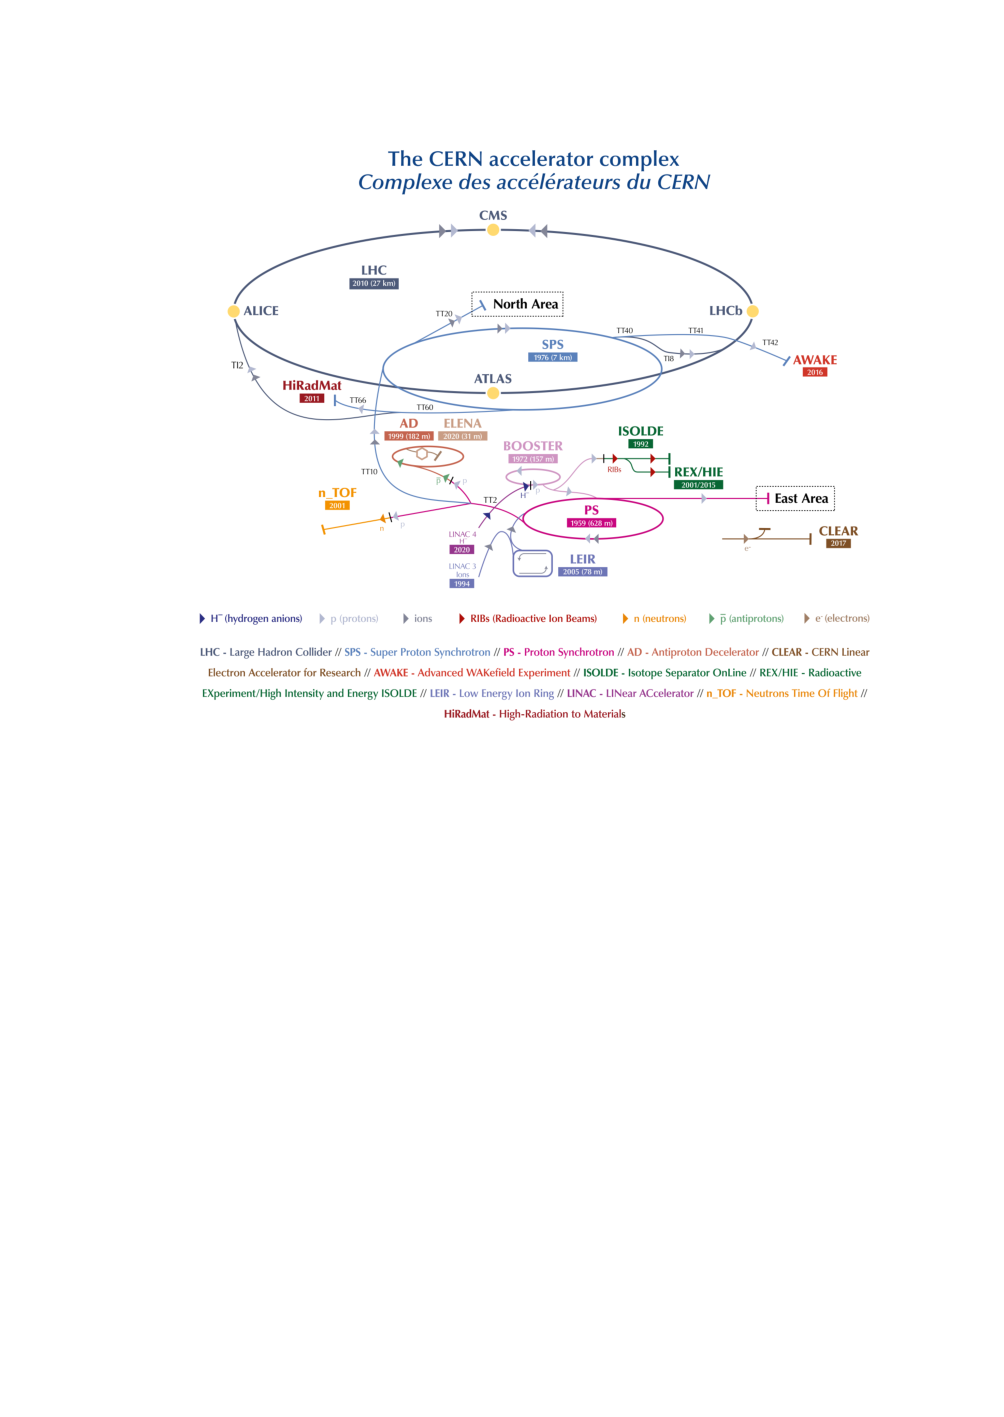
\includegraphics[width=1\linewidth]{images/CCC-v2022}\\
    \caption{Schematic overview of the CERN accelerator complex: the Large Hadron Collider, its injection chain and the four main experiments that record the collisions~\cite{Lopienska:2800984}.}
    \label{LHC:chain}
\end{figure}

For reference, the operation of the LHC is divided into distinct data-taking periods, known as Runs, which are separated by long shutdowns (LS) dedicated to maintenance and upgrades. Run-1 (2010--2012) delivered collisions at centre-of-mass energies of 7 and 8~TeV, culminating in the discovery of the Higgs boson. After the first long shutdown (LS1), Run-2 (2015--2018) resumed at 13~TeV, providing nearly 200~fb$^{-1}$~\footnote{Luminosity and its units are explained in next Section~\ref{subsec:lumi}} of data and enabling precision Higgs measurements as well as a broad programme of new physics searches. Following LS2 (2019--2021), Run-3 started in 2022 at 13.6~TeV and is expected to deliver about 300--500~fb$^{-1}$ of integrated luminosity. Looking further ahead, the High-Luminosity LHC (HL-LHC), scheduled to begin after LS3 around 2029, will increase the dataset by an order of magnitude, aiming for a total integrated luminosity of 3000--4000~fb$^{-1}$ at up to 14~TeV, thereby opening the door to unprecedented precision in Higgs and electroweak physics. The LHC/HL-HLC schedule is summarized in Figure~\ref{fig:LHC-HL}.

\begin{figure}[htbp]
    \centering
    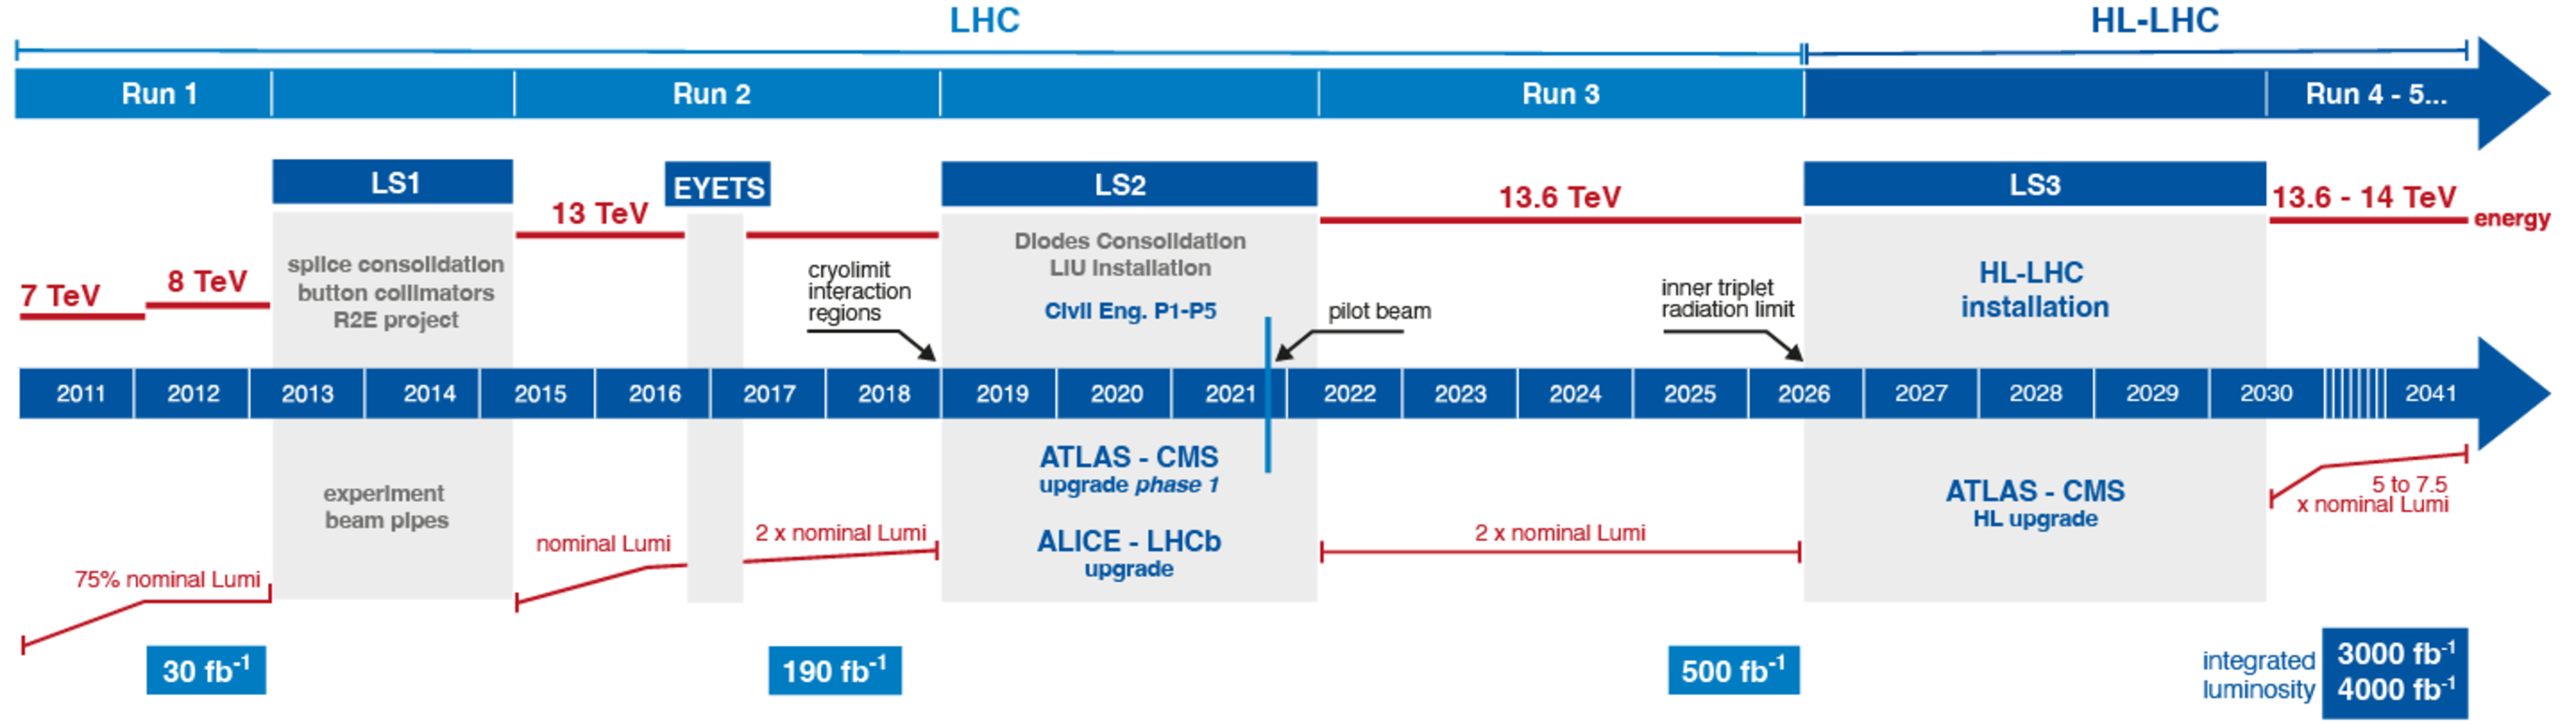
\includegraphics[width=1\linewidth]{images/HL-LHC_Plan_January2025.pdf}\\
    \caption{Timeline of the LHC operational Runs and the HL-LHC upgrade plan~\cite{HL-LHC_plans}.}
    \label{fig:LHC-HL}
\end{figure}


%xxxxxxxxxxxxxxxxxxxxxxxxxxxxxxxxxxxxxxxxxxxxxxxxxxxxxx
\subsection{Beam conditions and luminosity}
%xxxxxxxxxxxxxxxxxxxxxxxxxxxxxxxxxxxxxxxxxxxxxxxxxxxxxx
\label{subsec:lumi}
Besides the energy that LHC can deliver to the colliding protons, another important performance characteristic of the accelerator is the number of collision events that it can produce. If one considers the instantaneous luminosity as a measure of the particle flux, then in a scattering process such as proton-proton collisions, the number of collisions can be expressed as:

\begin{equation}
  N^{\text{proc}}_\text{{events}} = \sigma^{\text{proc}}_{\text{event}} \int L\text{d}t = \sigma^{\text{proc}}_{\text{event}}\mathcal{L},
\end{equation}
which is proportional to the cross-section representing the underlying physics of the process of interest, $\sigma^{\text{proc}}_{\text{event}}$, such as Higgs boson production. The time integral over the instantaneous luminosity is referred to as the integrated luminosity, $\mathcal{L}$. The instantaneous luminosity ($L$) depends on the properties of the beams and can be expressed as follows~\cite{Aad_2023}:
\begin{equation}
    L = f_{\text{rev}}\frac{N_1 N_2 N_b}{4\pi \sigma_x \sigma_y},
\end{equation}
where $N_b$ is the number of bunches per beam, $N_1$ and $N_2$ are the number of protons per bunch and $f_{\text{rev}}$ is the beam revolution frequency. In practice not all bunches are filled with electrons, and moreover these proton packs have extensions in both two directions perpendicular to the beam propagation direction assuming an effective gaussian shape with area $4\pi\sigma_{x}\sigma_{y}$, being $\sigma_{x}$ and $\sigma_{y}$ the horizontal and vertical gaussian widths respectively.  

The integrated luminosity is typically expressed in units of inverse femtobarns (fb$^{-1}$), where $1~\text{fb}^{-1} = 10^{39}~\text{cm}^{-2}$. Figure~\ref{figure:Run3lumi}(a) shows the integrated luminosity delivered to ATLAS for each year of data taking from 2011 to 2025. Figure~\ref{figure:Run3lumi}(b) displays a comparison between the cumulative luminosity delivered and recorded by the ATLAS detector during Run-2, which constitutes the main dataset analysed in this thesis, along with the early years of Run-3.

ATLAS collected approximately 147~fb$^{-1}$ of proton-proton collision data at a center-of-mass energy of 13~TeV during Run-2. However, not all delivered data are suitable for physics analysis. The dataset certified for physics-quality analyses, i.e.\ the one included in the Good Run List (GRL)~\cite{Aad_2020}, is slightly smaller due to quality and detector performance criteria. Specifically, ATLAS recorded a total of $140 \pm 1.2$~fb$^{-1}$ of high-quality data during Run-2, and approximately 166~fb$^{-1}$ during the years 2022--2024 of Run-3.

\begin{figure}[htbp]
\centering
\begin{tabular}{cc}
    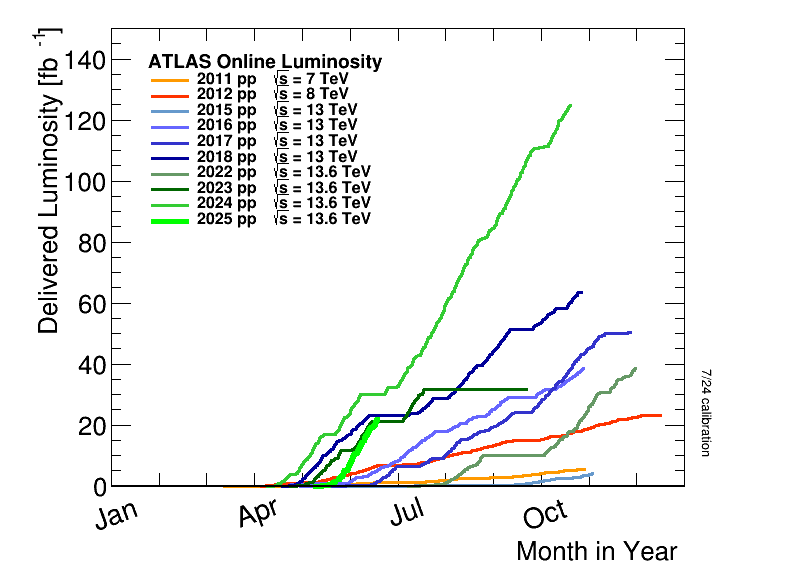
\includegraphics[width=0.5\linewidth]{images/intlumivsyear.png} &
    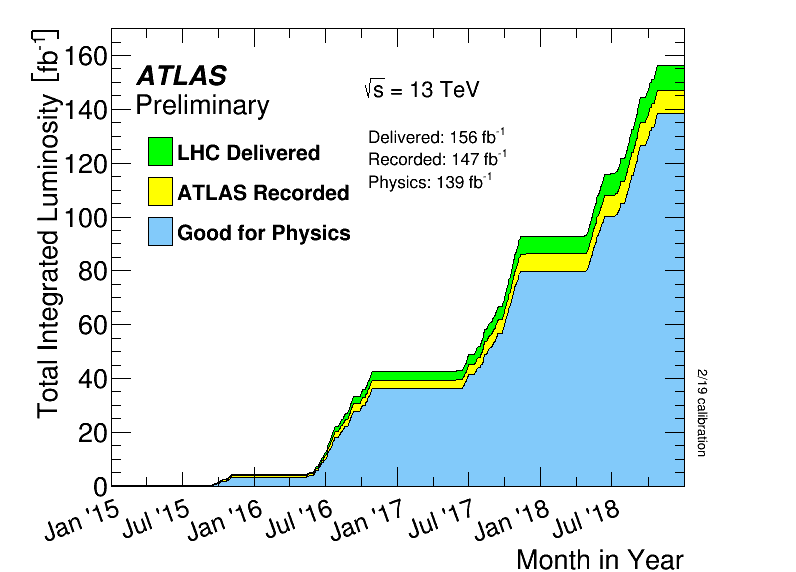
\includegraphics[width=0.5\linewidth]{images/intlumivstimeRun2DQall.png} \\
    (a) & (b)  \\
\end{tabular}
\caption{(a) Cumulative $pp$ collision luminosity delivered to the ATLAS detector as a function of the month
of the year, separately for years between 2011 and 2025~\cite{atlas:Run3lumi} and (b) cumulative luminosity versus
time delivered by the LHC (green), recorded by ATLAS (yellow) and used for physics (blue)
during stable beams for $pp$ collisions at 13 TeV centre-of-mass energy in years 2015-2018~\cite{atlas:Run2lumi}}
\label{figure:Run3lumi}
\end{figure}

%xxxxxxxxxxxxxxxxxxxxxxxxxxxxxxxxxxxxxxxxxxxxxxxxxxxxxx
\subsection{Pile-up and its challenges}
%xxxxxxxxxxxxxxxxxxxxxxxxxxxxxxxxxxxxxxxxxxxxxxxxxxxxxx

As previously mentioned, the proton bunches that collide at the various interaction points of the LHC contain a large number of protons. As a consequence, more than one hard proton-proton scattering commonly occur in a single bunch crossing. This phenomenon is known as pile-up.

More precisely, this effect is quantified with the average number of proton-proton interactions per bunch crossing to quantify this effect, since the number of interactions can vary depending on the beam conditions. Pile-up can be classified into two categories: in-time pile-up (which refers to multiple interactions occurring within the same bunch crossing) and out-of-time pile-up (which originates from proton-proton interactions taking place in neighboring bunch crossings). The latter can affect the measurements when the readout times of the detector systems exceed the time interval between consecutive bunches, complicating the identification of the primary vertex and the correct association of final-state particles to it.

The number of interactions per bunch crossing follows a Poisson distribution, with a mean value $\mu$ proportional to the product of the total inelastic proton-proton cross-section $\sigma_{\text{inel}}$ and the instantaneous luminosity~\cite{pileup}
\begin{equation}
    \mu = \frac{\text{L}\sigma_{\text{inel}}}{f_{\text{rev}}}.
\end{equation}
Figure~\ref{fig:pileup} shows the distribution of the mean number of interactions per bunch crossing in ATLAS during both Run-2 and Run-3.
Increasingly efforts are being devoted to develop mitigation strategies for this effect, including advanced pile-up suppression techniques such as vertex association, pile-up subtraction in jets and missing energy, and the use of machine learning algorithms to distinguish primary vertices from pile-up vertices~\cite{ATL-PHYS-PUB-2023-011,ATLAS:2017pfq,Soyez_2019}.
\begin{figure}[htbp]
    \centering
    \begin{tabular}{cc}
        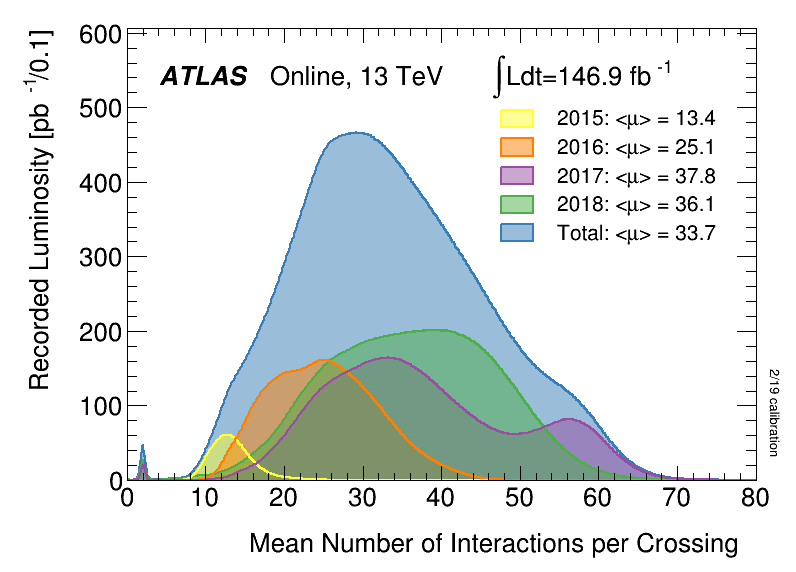
\includegraphics[width=0.5\linewidth]{images/mu_2015_2018.png} &
        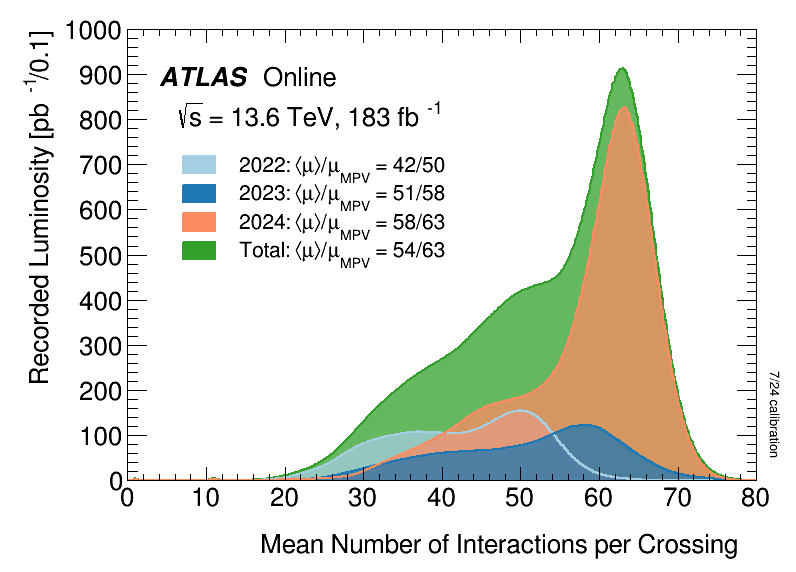
\includegraphics[width=0.5\linewidth]{images/mu_2022_2024.png} \\
        (a) & (b)  \\
    \end{tabular}
    \caption{(a) Distribution of mean number of interactions per bunch crossing in data recorded by the ATLAS experiment at 13~TeV during Run-2~\cite{atlas:Run2lumi} and  (b) at 13.6~TeV during Run-3~\cite{atlas:Run2lumi} data-taking periods.}
    \label{fig:pileup}
    \end{figure}
%xxxxxxxxxxxxxxxxxxxxxxxxxxxxxxxxxxxxxxxxxxxxxxxxxxxxxx
\subsection{LHC upgrade plans}
%xxxxxxxxxxxxxxxxxxxxxxxxxxxxxxxxxxxxxxxxxxxxxxxxxxxxxx

To further push the frontiers of high-energy physics and enhance the physics reach of the LHC programme, a major upgrade of the collider and its experiments is underway. The High-Luminosity LHC (HL-LHC) project~\cite{HLLHC} aims to increase the integrated luminosity delivered to the experiments by more than an order of magnitude, targeting up to 3000~fb$^{-1}$ of proton-proton collision data by the end of the next decade.

This increase in data volume will significantly improve the statistical precision of measurements of rare processes and enable detailed studies of the Higgs boson properties, electroweak interactions, and potential signals of BSM physics. In particular, the HL-LHC will allow for precise measurements of Higgs boson couplings, self-interactions, and rare decays, as well as the potential observation of extremely suppressed processes such as flavour-violating decays or double Higgs production.

Achieving the HL-LHC goals requires a broad range of upgrades to the accelerator complex and its associated infrastructure. Key improvements include the installation of new high-field superconducting quadrupole magnets near the interaction points, based on advanced Nb$_3$Sn technology~\cite{Mangiarotti:2770766}, which will allow for a reduction in the beams width, and consequently, an increase in luminosity. Additionally, new cryogenic and collimation systems will be implemented to handle the increased beam power and radiation levels.

On the experiment side, all main LHC experiments, including ATLAS, are undergoing substantial upgrades to handle the harsher conditions of HL-LHC operation. These include the development of new inner trackers with extended radiation hardness and granularity, the replacement of calorimeter and muon chamber readout electronics to support higher data rates, and a completely redesigned trigger and data acquisition system. The upgraded detectors must be capable of maintaining excellent performance in the presence of average pile-up levels exceeding $\langle\mu\rangle \sim 140$, more than a factor of two higher than those typically encountered during Run-3.

As shown in Figure~\ref{fig:LHC-HL}, the HL-LHC project is expected to start operations by 2030, following the completion of the Long Shutdown 3 (LS3). It represents the next major milestone in the LHC physics programme, with the potential to open a new era of precision measurements and exploration of the unknown.


%++++++++++++++++++++++++++++++++++++++++++++++
\section{The ATLAS detector}
\label{sec:ATLAS}
%++++++++++++++++++++++++++++++++++++++++++++++

Having already outlined the LHC design, physics programme and scientific goals, this section presents in detail each of the main components of the ATLAS experiment.

ATLAS~\cite{ATLAS:exp,ATLAS_run3} is a general-purpose detector designed to explore a wide spectrum of physics phenomena, ranging from precision tests of the SM to searches for new particles and interactions beyond it. It is the largest 
detector ever constructed for a collider experiment, with a cylindrical geometry approximately 44~m long, 25~m diameter, and weighing over 7000~tons. Its conception, design and construction were carried out by a global collaboration of more than 5000 scientists and engineers from around 180 institutions in nearly 40 countries.

The ATLAS detector is composed of multiple subdetectors arranged in concentric layers 
around the interaction point. The cylindrical structure is closed by two end-caps, providing almost $4\pi$ coverage of the solid angle. An illustration of the ATLAS detector can be found in Figure~\ref{fig:ATLASdet}.

The different ATLAS subsystems are designed to measure the properties of different types of particles. In the innermost region, closest to the interaction point, the inner detector is built to record the properties of charged particles produced in the collisions. Their trajectories 
are bent by a 2~T magnetic field produced by a superconducting solenoid. Then, the inner detector is surrounded by the calorimeter system, which measures the energy of particles producing electromagnetic and hadronic showers. This system consists of a liquid-argon electromagnetic calorimeter and a hadronic calorimeter with a scintillating barrel and liquid-argon end-caps.
In the outermost region of the detector it is placed the muon spectrometer, devoted to the measurement of muons produced in the collision and which are bent by a 0.5-1~T magnetic field produced by a toroidal magnet system.
The following sections describenthe purpose and operating principles of these components, as well as the forward detectors, the trigger and data acquisition systems.

\begin{figure}[htbp]
    \centering
        \includegraphics[width=1\linewidth]{ATLAS-Experiment-Schematic-2022-Labels-People.png}
    \caption{Cut-away view of the Run-3 configuration of the ATLAS detector indicating the locations of the larger detector subsystems~\cite{Bianchi:2837191}.}
    \label{fig:ATLASdet}
\end{figure}

%xxxxxxxxxxxxxxxxxxxxxxxxxxxxxxxxxxxxxxxxxxxxxxxxxxxxxx
\subsection{Reference frame and coordinate system}
\label{sec:coordinates}
%xxxxxxxxxxxxxxxxxxxxxxxxxxxxxxxxxxxxxxxxxxxxxxxxxxxxxx

The ATLAS experiment adopts a right-handed coordinate system, centered at the nominal interaction point where the proton-proton collisions take place, as seen in Figure~\ref{fig:coord}. The origin of the coordinate system lies at the geometrical center of the detector. The $z$-axis is defined along the beam pipe, pointing in the direction of the anti-clockwise beam. The $x$-axis points from the IP towards the center of the LHC ring, while the $y$-axis points upwards, 
completing a right-handed coordinate system. The transverse plane defined by $x$ and $y$ directions is used to define important observables like the transverse momentum ($p_{\text{T}}$) and the so-called missing transverse momentum ($E^{\text{miss}}_{\text{T}}$).

In addition to the Cartesian coordinates $(x, y, z)$, a cylindrical coordinate system is often used due to the symmetry of the detector. In this system, the transverse plane is defined by the coordinates $(r, \phi)$, where $r$ is the radial distance from the $z$-axis and $\phi$ is the azimuthal angle measured around the beam pipe. The longitudinal direction remains aligned with the $z$-axis.

To describe the polar angle of a particle’s trajectory, defining deviations from the beam direction, the rapidity ($y$) is preferred over the polar angle $\theta$, as it is invariant under Lorentz boosts along the $z$-axis:
\begin{equation}
    y = \frac{1}{2}\ln{\frac{E+p_{z}}{E-{p_{z}}}},
\end{equation}
where $E$ is the particle's energy and $p_{z}$ the longitudinal component of its momentum. In the ultra-relativistic limit, this variable can be approximated by the so-called pseudorapidity ($\eta$), since the mass of most of final-state particles is mostly negligible against their momenta:
\begin{equation}
\eta = -\ln \tan \left( \frac{\theta}{2} \right).
\end{equation}
In this frame, if a particle is emmitted in the beam direction, $\theta \rightarrow 0º$, it would have assigned $\eta \rightarrow \infty$, while if it follows a direction perpendicular to the beam, $\theta = 90º$ corresponds to $\eta = 0$.
The angular separation between two objects in the detector is typically measured using the $\Delta R$ metric in the $(\eta, \phi)$ plane:
\begin{equation}
\Delta R = \sqrt{(\Delta \eta)^2 + (\Delta \phi)^2}.
\end{equation}
which can also be computed directly from the rapidity $y$.

This coordinate convention is used throughout the analysis and the design of the detector subcomponents, as well as in reconstruction and identification algorithms for physics objects such as jets, leptons, and missing transverse energy.
\begin{figure}[t]
    \centering
        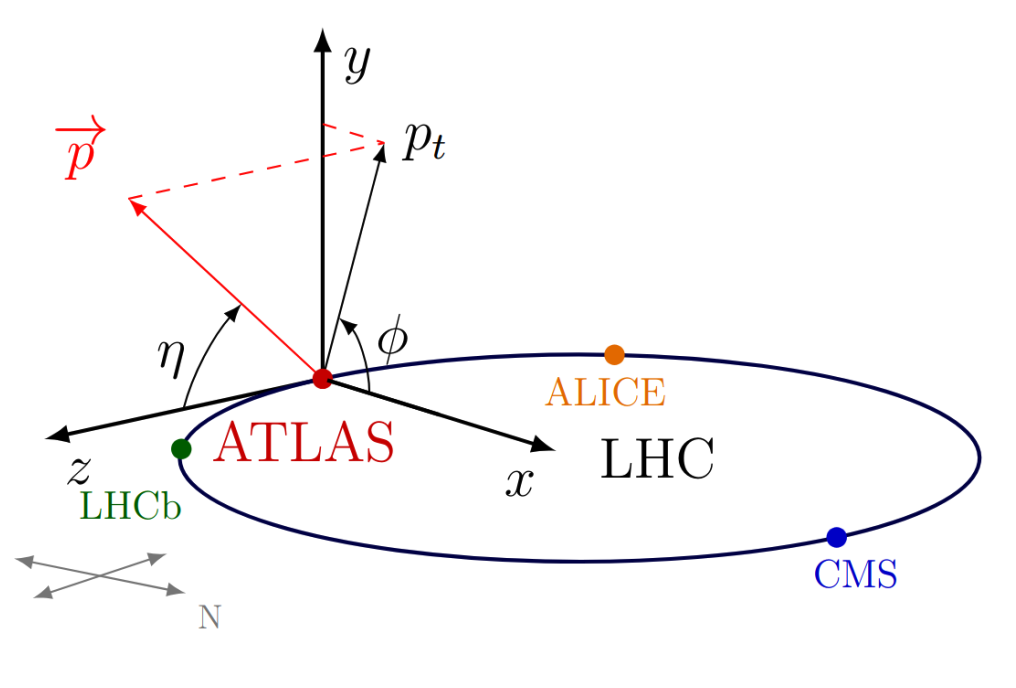
\includegraphics[width=0.6\linewidth]{ATLAS_coordinates.png}
    \caption{Illustration of the ATLAS coordinate system. Image obtained from Ref.~\cite{coordinates}.}
    \label{fig:coord}
\end{figure}

%xxxxxxxxxxxxxxxxxxxxxxxxxxxxxxxxxxxxxxxxxxxxxxxxxxxxxx
\subsection{Inner detector}
\label{sec:ID}
%xxxxxxxxxxxxxxxxxxxxxxxxxxxxxxxxxxxxxxxxxxxxxxxxxxxxxx


The Inner Detector (ID)~\cite{2010_id,ATLAS:exp} is the central tracking system of the ATLAS experiment and plays a fundamental role in the reconstruction of charged particles emerging from proton-proton collisions. It is the innermost component of the detector, positioned directly around the interaction point. 

The ID is composed of three complementary subdetectors arranged in layers from the innermost to the outermost radii: the Pixel Detector, the Semiconductor Tracker (SCT), and the Transition Radiation Tracker (TRT). An schematic view of the barrel section of the ID can be found in Figure~\ref{fig:id}.
The Pixel and SCT systems are based on silicon technologies and are optimized for high spatial resolution and precision tracking. In contrast, the TRT is a gaseous detector made of straw tubes and is designed to extend the tracking capabilities at higher radii while also enhancing electron identification through the detection of transition radiation.

Together, these three subdetectors span a cylindrical volume of approximately 6.2~m in length and 2.1~m in diameter, and provide tracking coverage in the pseudorapidity range of $|\eta| < 2.5$. The layout of the ID is divided into a central barrel region ($|\eta| < 1.4$) and two symmetric endcap sections ($1.4 < |\eta| < 2.5$). As charged particles traverse the ID, they produce hits in the different layers, which are then used to reconstruct their trajectories with high efficiency and resolution. 
These reconstructed trajectories, referred to as \textit{tracks}, represent the paths of charged particles through the detector and constitute the essential input for identifying not only primary vertices (which are the spatial locations where the hard scattering of partons of interest in a given event took place) but also from other vertices that are displaced from the primary one and could originate from the decay of heavy-flavour hadrons that travels enough before decaying. This is clearly essential for tagging of these jets, and supporting particle identification algorithms throughout the ATLAS reconstruction chain, as will be explained in Chapter~\ref{chap:object_rec}.
\begin{figure}[htbp]
    \centering
        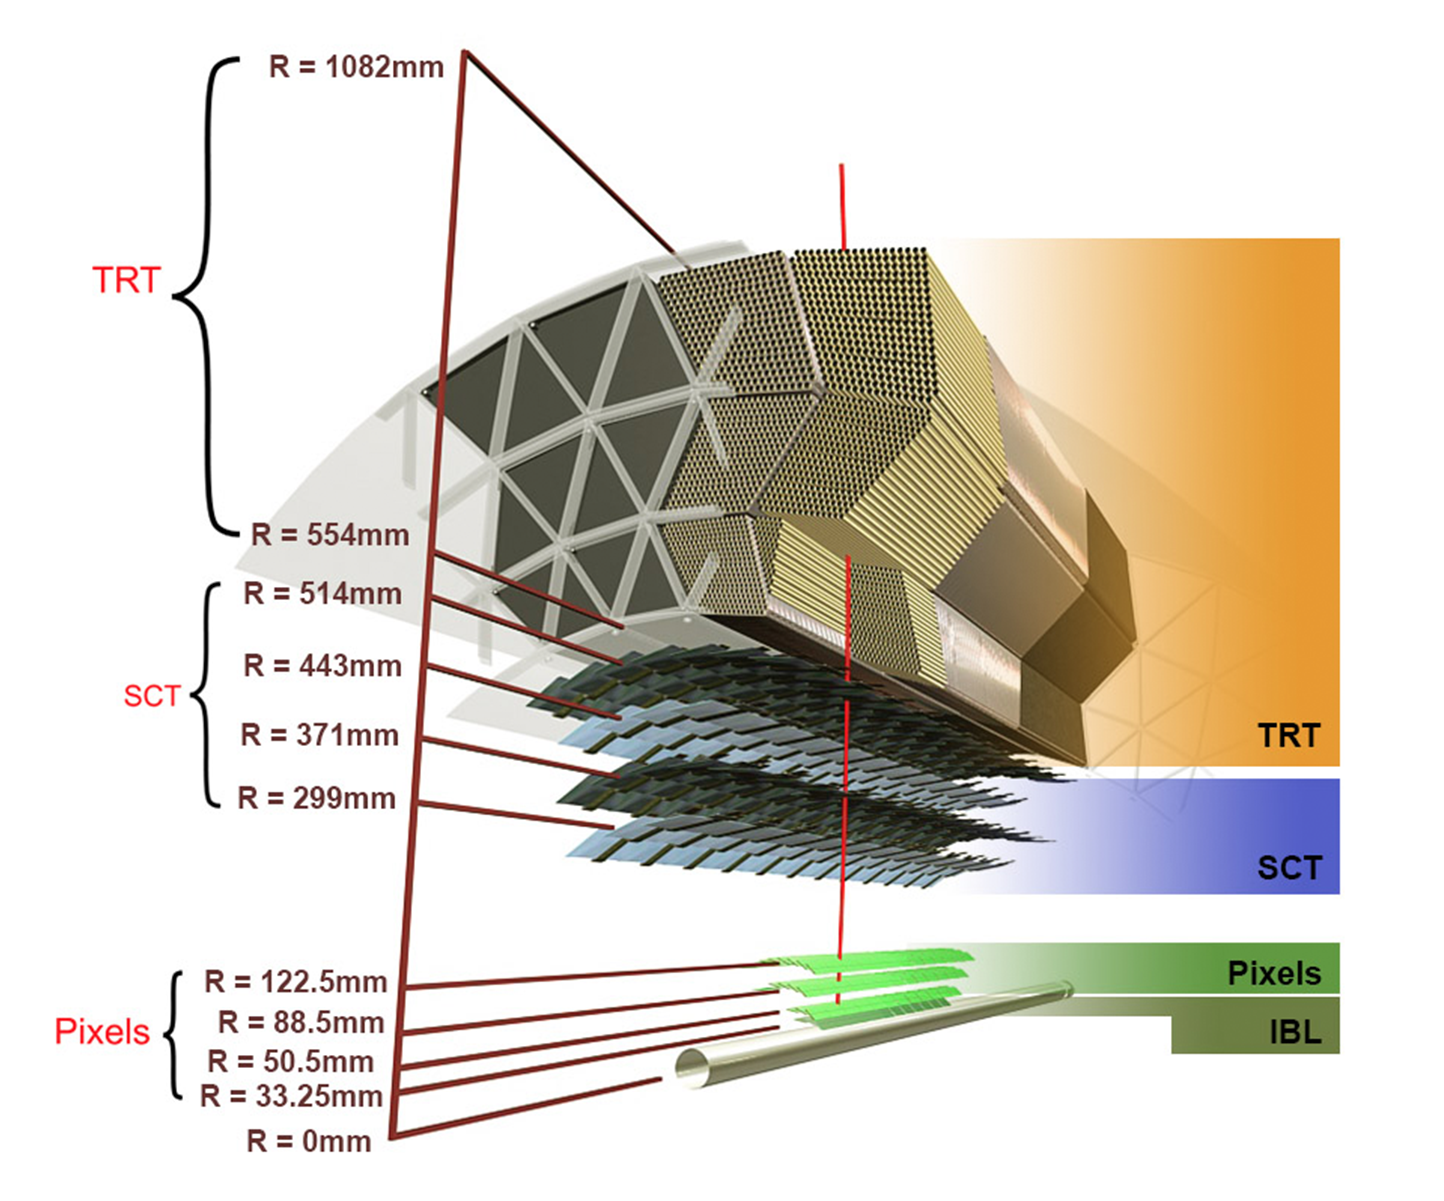
\includegraphics[width=0.7\linewidth]{ATLAS_id.png}
    \caption{Cutaway representation of the barrel section of the ATLAS inner detector. From the innermost to the outermost layers, it shows the pixel detector, the four cylindrical an concentrical layer of the SCR and the straw tubes characteristic of the TRT~\cite{Collaboration:2723878}.}
    \label{fig:id}
\end{figure}

\subsubsection*{Pixel detector}

The Pixel Detector is the innermost and most granular component of the ID. Its layout consists of three cylindrical layers of silicon pixel sensors in the barrel region, positioned at radial distances of 50.5, 88.5, and 122.5~mm, and three disks per endcap located at $z = \pm$495, 580, and 650~mm. The sensors in these layers have pixel sizes of $50 \times 400~\mu\text{m}^2$ and a thickness of 250~$\mu$m. This geometry yields a spatial resolution of about $10~\mu$m in the $r\text{--}\phi$ plane and $115~\mu$m in $z$ for the barrel region, and the opposite in the endcaps, where resolution is optimized along $z$.

In preparation for Run-2, an additional innermost layer known as the Insertable B-Layer (IBL)~\cite{IBL} was installed at a radius of 33.25~mm. The IBL significantly improved the impact parameter resolution, particularly for low-$p_{\mathrm{T}}$ tracks. It is composed of both planar and 3D silicon sensors with reduced pixel dimensions of $50 \times 250~\mu\text{m}^2$ and sensor thicknesses of 250~$\mu$m and 200~$\mu$m, respectively. The closer proximity of the IBL to the beamline and its finer segmentation improves its ability to separate primary and secondary vertices even under high occupancy conditions, which is crucial for the identification of jets originating from heavy-flavour quarks.

%During Run-3, the Pixel Detector has been operating under increasingly harsh radiation environments and elevated levels of pile-up. These conditions challenge the performance and life-time of the system, especially the innermost layers. Dedicated calibration and alignment strategies, as well as enhanced readout electronics, are employed to preserve the resolution and efficiency of tracking throughout this demanding phase of operation.

\subsubsection*{Semiconductor Tracker (SCT)}

Outwards, the SCT subdetector follows the pixel one, consisting of four barrel layers and nine disks in each endcap, built with silicon microstrip modules. Each module includes two sensors, mounted back-to-back at a small stereo angle of 40 mrad, enabling precise three-dimensional position reconstruction of $17$~$\mu$m resolution in the transverse plane and $580$~$\mu$m in the longitudinal direction. 
The SCT contains around 6 million readout channels.

\subsubsection*{Transition Radiation Tracker (TRT)}

The TRT is the outermost component of the Inner Detector and extends tracking capabilities up to $|\eta| < 2.0$, complementing the precise position measurements from the inner silicon detectors with additional points along the track path. The TRT also provides particle identification (PID) capabilities, particularly useful for electron-pion discrimination via detection of transition radiation photons.

It consists of a large number of thin straw tubes, 52,544 in the barrel region and 122,880 in the two endcaps, each with a diameter of 4~mm. These tubes are originally filled with a gas mixture of 70\% xenon, 27\% carbon dioxide, and 3\% oxygen. When a charged particle traverses a straw, it ionizes the gas along its path. A high negative voltage applied to the tube walls causes the liberated electrons to drift toward a central anode wire, producing a detectable signal. 

The TRT delivers a spatial resolution of approximately $130~\mu\text{m}$ in the $r\text{--}\phi$ plane and contributes on average about 30 measurement points per track, thus enhancing the momentum resolution and the track reconstruction efficiency, especially for high-$|\eta|$ regions where fewer silicon hits are available. Its ability to identify transition radiation, photons emitted by relativistic electrons crossing dielectric boundaries embedded in the tracker, provides an additional layer of particle identification crucial for several physics analyses.

During Run-3, it has been used an argon-based gas mixture in the entire barrel and part of the end-cap region to minimize xenon loss and ensure gas mixture stability. Although this reduces the barrel's PID performance due to weaker transition radiation photon absorption, it still provides useful electron identification when combined with the information from the ionization energy loss per unit length, d$E$/d$x$. The end-cap PID performance remains largely preserved~\cite{ATLAS_run3}.

%\vspace{-0.3}
%At this stage it is worth noting that, ahead of Run-3, an important part of the read-out electronics in several sub-detectors were refurbished and optimised to withstand the higher data rates expected during this period. By the end of Run-3 the existing silicon trackers will be operating close to their radiation-tolerance limits, and the TRT will no longer be able to function under the nominal HL-LHC conditions. To preserve vertex-tagging and track-reconstruction performance, the entire Inner Detector will therefore be superseded by an all-silicon Inner Tracker (ITk). In addition, a High-Granularity Timing Detector will be installed in the forward region in order to match tracks with calorimeter clusters using precise time information, that is an essential tool for mitigating the extreme pile-up foreseen at the HL-LHC \cite{ATLAS:1502664}
%xxxxxxxxxxxxxxxxxxxxxxxxxxxxxxxxxxxxxxxxxxxxxxxxxxxxxx
\subsection{Calorimeters}
\label{sec:calo}
%xxxxxxxxxxxxxxxxxxxxxxxxxxxxxxxxxxxxxxxxxxxxxxxxxxxxxx
The ATLAS calorimeter system~\cite{2010_lar,2010_tile} is located outside the solenoid magnet hosting the ID. Both types of calorimeters, electromagnetic and hadronic, cover a total range up to $|\eta| < 4.9$, allowing for the measurement of the energy of particles traversing them, 
as they are designed to completely absorb the energy of most particles except for muons and neutrinos. An schematic illustration of the ATLAS calorimeter system is shown in Figure~\ref{fig:cal}.
\begin{figure}[htbp]
    \centering
        \includegraphics[width=0.9\linewidth]{ATLAS_cal.png}
    \caption{Cutaway representation of the ATLAS calorimeter system and its main components~\cite{ATLAS_run3}.}
    \label{fig:cal}
\end{figure}

%%%%%%%%%%%%%%%%%%%%%%%%%%%%%%%
\subsubsection{LAr electromagnetic calorimeter}
\label{sec:elelar}
%%%%%%%%%%%%%%%%%%%%%%%%%%%%%%%

The electromagnetic (EM) calorimeter in the ATLAS detector is designed to precisely measure the energy of electrons and photons. It is based on a sampling technology that uses LAr as the active medium and different metals (either tungsten, copper or lead) as the absorber material. This choice combines a high level of granularity with excellent linearity and radiation hardness, crucial for operation in the high-luminosity environment of the LHC.

The EM calorimeter is divided into three main regions: a barrel section covering the pseudorapidity range $|\eta| < 1.475$ (EMB), and two end-cap sections (EMEC) that extend the coverage up to $|\eta| = 3.2$. Each region is segmented longitudinally into three layers plus a presampler, as can be seen in Figure~\ref{fig:LAr_EM}, optimizing the reconstruction of electromagnetic showers. The presampler layer is used to correct for energy loss in the material upstream of the calorimeter. The first layer features fine granularity in the $\eta$ direction ($\Delta\eta = 0.0031$), allowing for precise discrimination between single photons and pairs of close-by photons resulting from neutral pion decays. The second layer collects most of the energy from electromagnetic showers and provides the primary energy measurement. The third layer corrects for energy leakage at high energies.

\begin{figure}[htbp]
    \centering
        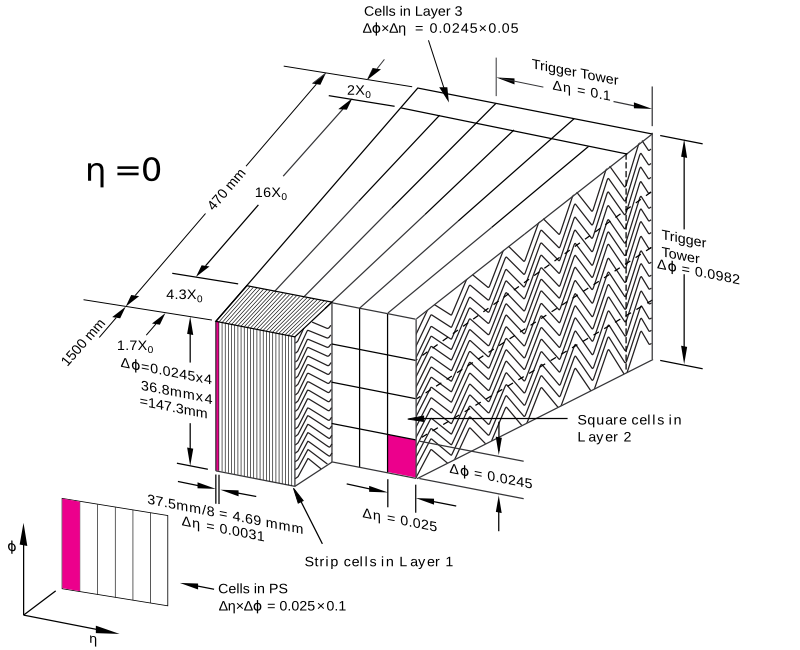
\includegraphics[width=0.75\linewidth]{LAr_EM.png}
    \caption{Schematic diagram of the cross-section of the LAr EM barrel calorimeter, including the presampler. The different granularity in $\eta$ and $\phi$ of the cells of each of the three layers is also shown~\cite{ATLAS:exp}}
    \label{fig:LAr_EM}
\end{figure}

The EM LAr calorimeter employs an accordion-shaped geometry in both the barrel and end-cap regions. This design ensures full azimuthal coverage without projective cracks, while maintaining uniform response and mechanical stability. The calorimeter modules are housed in cryostats filled with liquid argon, operating at a temperature of approximately 87~K. The readout cells are segmented into towers of size $\Delta\eta \times \Delta\phi = 0.025 \times 0.025$ in the second layer, which defines the granularity for standard electromagnetic object reconstruction.

The signal is induced by the LAr ionization caused by charged particles in the shower. Ionization electrons drift under a high-voltage electric field, and the resulting current is read out with high precision using fast low-noise electronics, allowing the determination of the energy deposited by the original particle that hit the detector. In calorimetry, the typical energy resolution is generally expressed as
\begin{equation}
\frac{\sigma_E}{E} = \frac{a}{\sqrt{E}} \oplus b \oplus \frac{c}{E},
\end{equation}
where $E$ denotes the particle energy measured in GeV, and $\sigma_E$ its associated resolution. This parametrization is universal in calorimetry: the first term, $a/\sqrt{E}$, represents the stochastic contribution (about $10\%$ for the ATLAS EM calorimeter), the second term $b$ is a constant term (below $0.7\%$), and the last term $c/E$ accounts for the contribution from electronic noise. The excellent performance of the ATLAS electromagnetic calorimeter, following this general behaviour, is essential for precision measurements such as the $H \rightarrow \gamma\gamma$ and $H \rightarrow ZZ^* \rightarrow 4\ell$ channels.

%%%%%%%%%%%%%%%%%%%%%%%%%%%%%%%
\subsubsection{LAr hadronic calorimeters}
\label{sec:elehad}
%%%%%%%%%%%%%%%%%%%%%%%%%%%%%%%

The hadronic calorimeter system complements the electromagnetic calorimeter by measuring the energy of hadrons. In the end-cap and forward regions, the hadronic calorimetry is provided by these LAr-based detectors: the Hadronic End-Cap Calorimeter (HEC) and the Forward Calorimeter (FCal).

The HEC is positioned directly behind the EMEC and covers the pseudorapidity range $1.5 < |\eta| < 3.2$. It consists of copper plates as absorbers and uses liquid argon as the active medium. The copper-LAr combination ensures a compact structure with good radiation hardness and linearity. The HEC is segmented longitudinally into four layers and, together with the electromagnetic calorimeter, provides sufficient depth to ensure efficient containment of hadronic showers. Each end-cap consists of two wheels: a front wheel (HEC1) constituted of 24 copper plates, and a rear wheel (HEC2) made of 16 copper plates.

The Forward Calorimeter (FCal) extends the coverage to $|\eta| < 4.9$ and is composed of three longitudinal modules: the first is electromagnetic, featuring copper absorbers, and the second and third modules are hadronic, and uses tungsten absorbers in order to reduce the lateral spread of the hadronic showers. The high-density design of the FCal is necessary to withstand the high particle flux and radiation levels encountered in the forward region. Due to its crucial role in reconstructing the forward energy flow, the FCal is also essential for pile-up suppression and missing transverse energy reconstruction.

Both HEC and FCal calorimeters operate within the same LAr cryostats as the electromagnetic sections, benefitting from the same stability and fast response. 

%%%%%%%%%%%%%%%%%%%%%%%%%%%%%%%
\subsubsection{Hadronic Tile calorimeter}
\label{sec:tilecal}
%%%%%%%%%%%%%%%%%%%%%%%%%%%%%%%

The Tile Calorimeter (TileCal) is ATLAS main hadronic calorimeter, constructed as a sampling calorimeter composed of alternating layers of plastic scintillator tiles (active material) and low-carbon steel absorber plates. Positioned around the LAr EM calorimeter, TileCal provides coverage in the pseudorapidity region $|\eta|<1.7$ and ensures containment of hadronic showers, limiting punch-through to the muon system.

TileCal consists of a central long barrel (LB) section ($|\eta|<1.0$, length of 5.8 m) and two extended barrel (EB) sections (EBA and EBC), each covering $0.8<|\eta|<1.7$ with a length of 2.6 m.

Each barrel segment is divided into 64 modules, featuring alternating 3 mm thick scintillator tiles and 14 mm thick steel absorbers along the beam axis. The scintillator tiles, arranged radially in 11 rows, generate scintillation light upon particle interaction. Wavelength-shifting fibers collect and shift this light to longer wavelengths, guiding it to photomultiplier tubes at the module's outer radius, enabling efficient and hermetic readout.

The calorimeter modules are segmented into three longitudinal layers: layers A, BC, and D in the LB, and layers A, B, and D in the EB. Cells in these layers have granularity of $\Delta\eta \times \Delta\phi=0.1\times0.1$ for inner layers and $0.2\times0.1$ for the D layers.

Additionally, gap scintillator cells were installed between TileCal and LAr to correct for energy losses and enhance performance. The Minimum-Bias Trigger Scintillators (MBTs), also read out by TileCal electronics, provide coverage in $2.08<|\eta|<3.86$ for triggering purposes. Overall, TileCal incorporates 9852 readout channels, covering 5182 cells.

Figure~\ref{fig:cal_resum} shows an schematic view of the readout geometry of all the calorimeter systems in the $r$--$z$ space, showing the different $\eta$ ranges covered by them and their segmentation.
\begin{figure}[htbp]
    \centering
        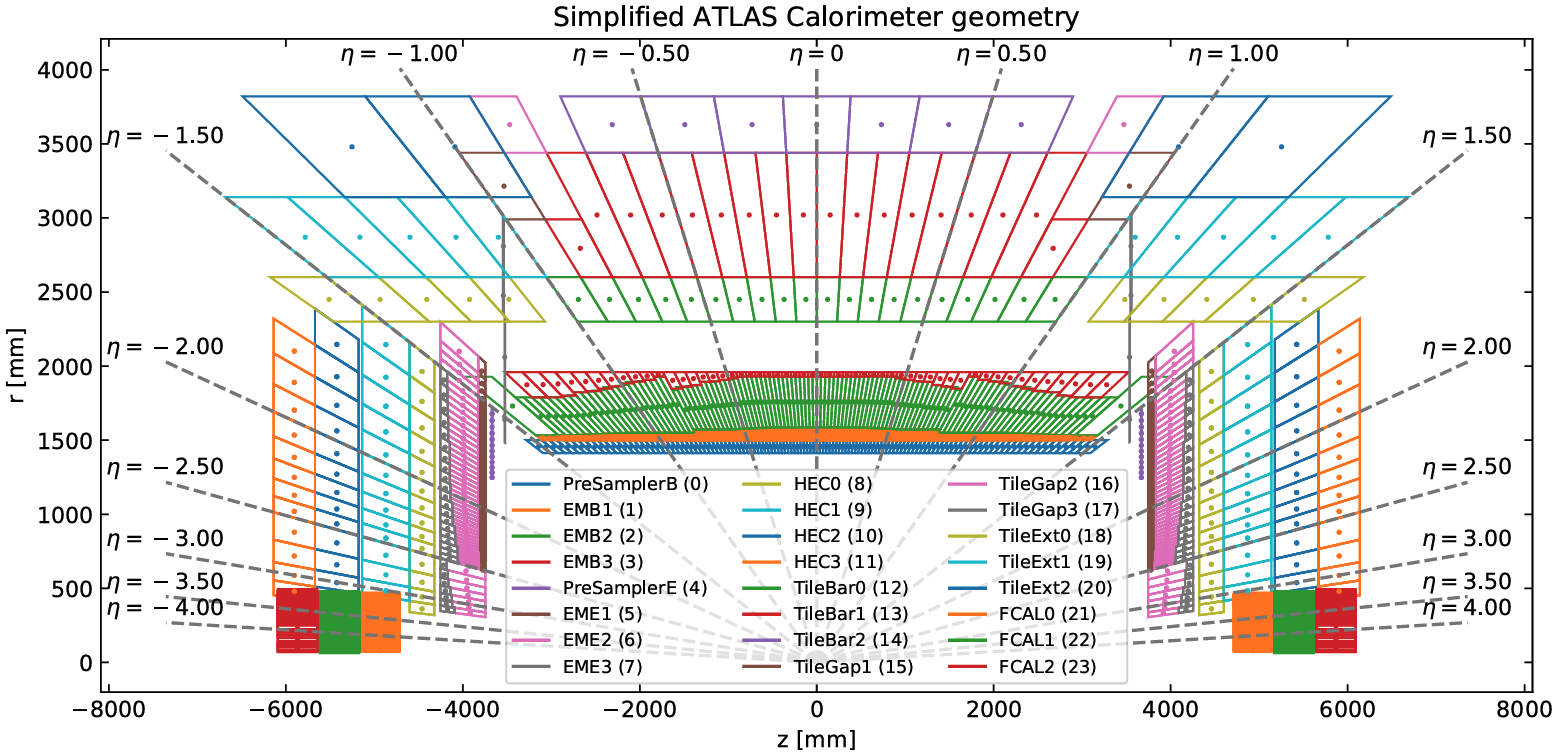
\includegraphics[width=0.95\linewidth]{cal_readout_ATLAS.png}
    \caption{Visualization of the ATLAS calorimeter readout geometry. The four subsystems, LAr EM, HEC, FCal and TileCal, and the layers of their segmentation are shown~\cite{Gessinger:2752944}.}
    \label{fig:cal_resum}
\end{figure}

%\vspace{-0.3}

%Additional upgrades have also been implemented in the ATLAS calorimeter electronics to meet Run-3 conditions and to prepare for the forthcoming HL-LHC era, mirroring the improvements made to the Inner Detector and ensuring compatibility with the new trigger architecture. Both the Liquid-Argon and Tile Calorimeters have refurbished their on-detector and off-detector read-out chains; in TileCal specifically, new scintillating cryostat counters and renewed Minimum-Bias Trigger Scintillators have been installed for Run-3, enhancing electron-energy resolution and improving luminosity monitoring.

%xxxxxxxxxxxxxxxxxxxxxxxxxxxxxxxxxxxxxxxxxxxxxxxxxxxxxx
\subsection{Muon spectrometer}
\label{sec:muon}
%xxxxxxxxxxxxxxxxxxxxxxxxxxxxxxxxxxxxxxxxxxxxxxxxxxxxxx


Figure~\ref{fig:ms_atlas} shows the outermost subsystem of ATLAS, known as the Muon Spectrometer (MS)~\cite{muon_com}, which is responsible for identifying muons, particles capable of traversing the calorimetric system with minimal energy loss. The MS comprises precision tracking chambers and fast-response trigger detectors embedded in a magnetic field of approximately 0.5~T in the barrel and 1.0~T in the end-cap regions, bending the trajectories of muons and enabling precise momentum measurement.

Four detector technologies totaling over one million readout channels are included in the MS. Resistive Plate Chambers (RPCs) are used in the barrel region ($|\eta| < 1.05$), providing measurements with a resolution of about 10~mm in both longitudinal and transverse directions. In the end-cap region ($1.05 < |\eta| < 2.4$), Thin Gap Chambers (TGCs) handle higher background rates with wire separation of 1.8~mm and positional resolution around 5~mm. The RPC and TGC detectors primarily function as triggering components due to their fast response times.

Precision muon tracking relies mainly on Monitored Drift Tubes (MDTs), installed in both barrel and end-cap regions, covering the range $|\eta| < 2.7$ and offering high positional accuracy (approximately 35~µm per chamber). Cathode Strip Chambers (CSCs), multi-wire proportional chambers providing high rate capability and excellent time resolution (4~ns), are employed in the forward region ($2.0 < |\eta| < 2.7$). MDTs and CSCs are critical for accurately reconstructing muon trajectories.

For Run-3, the MS underwent significant upgrades, including the replacement of the forward muon-tracking region (known as the small wheel) with the New Small Wheel (NSW)~\cite{nsw_tech}. The NSW consists of two large 100-ton units detectors located at each end of ATLAS, each 10 metres in diameter and segmented into 16 sectors. The NSW employs advanced detector technologies such as Micromegas (MM) and small-strip Thin Gap Chambers (sTGC), capable of simultaneous precision tracking and triggering. Each wheel contains two layers of MM and sTGC chambers, resulting in four measurement planes for improved tracking accuracy and more than 2 million readout channels.

%Moreover, despite being primarily designed to detect muons, the MS occasionally detects punch-through jets, hadronic jets that are not entirely absorbed by the calorimeters and reach the MS. 
The upgraded configuration of the MS, particularly with the addition of the NSW, significantly enhances ATLAS' capabilities in terms of tracking precision and trigger efficiency, essential for the high luminosity and challenging conditions expected during Run-3 and beyond.

%Furthermore and aiming HL-LHC era, The Muon detectors will install new chambers in the barrel (RPCs and MDTs), replace the TGCs in the gap between the barrel and the end-caps and upgrade the readout electronics for the already installed RPCs, TGCs and MDTs to make them fully compatible with the trigger architecture.

\begin{figure}[htbp]
    \centering
        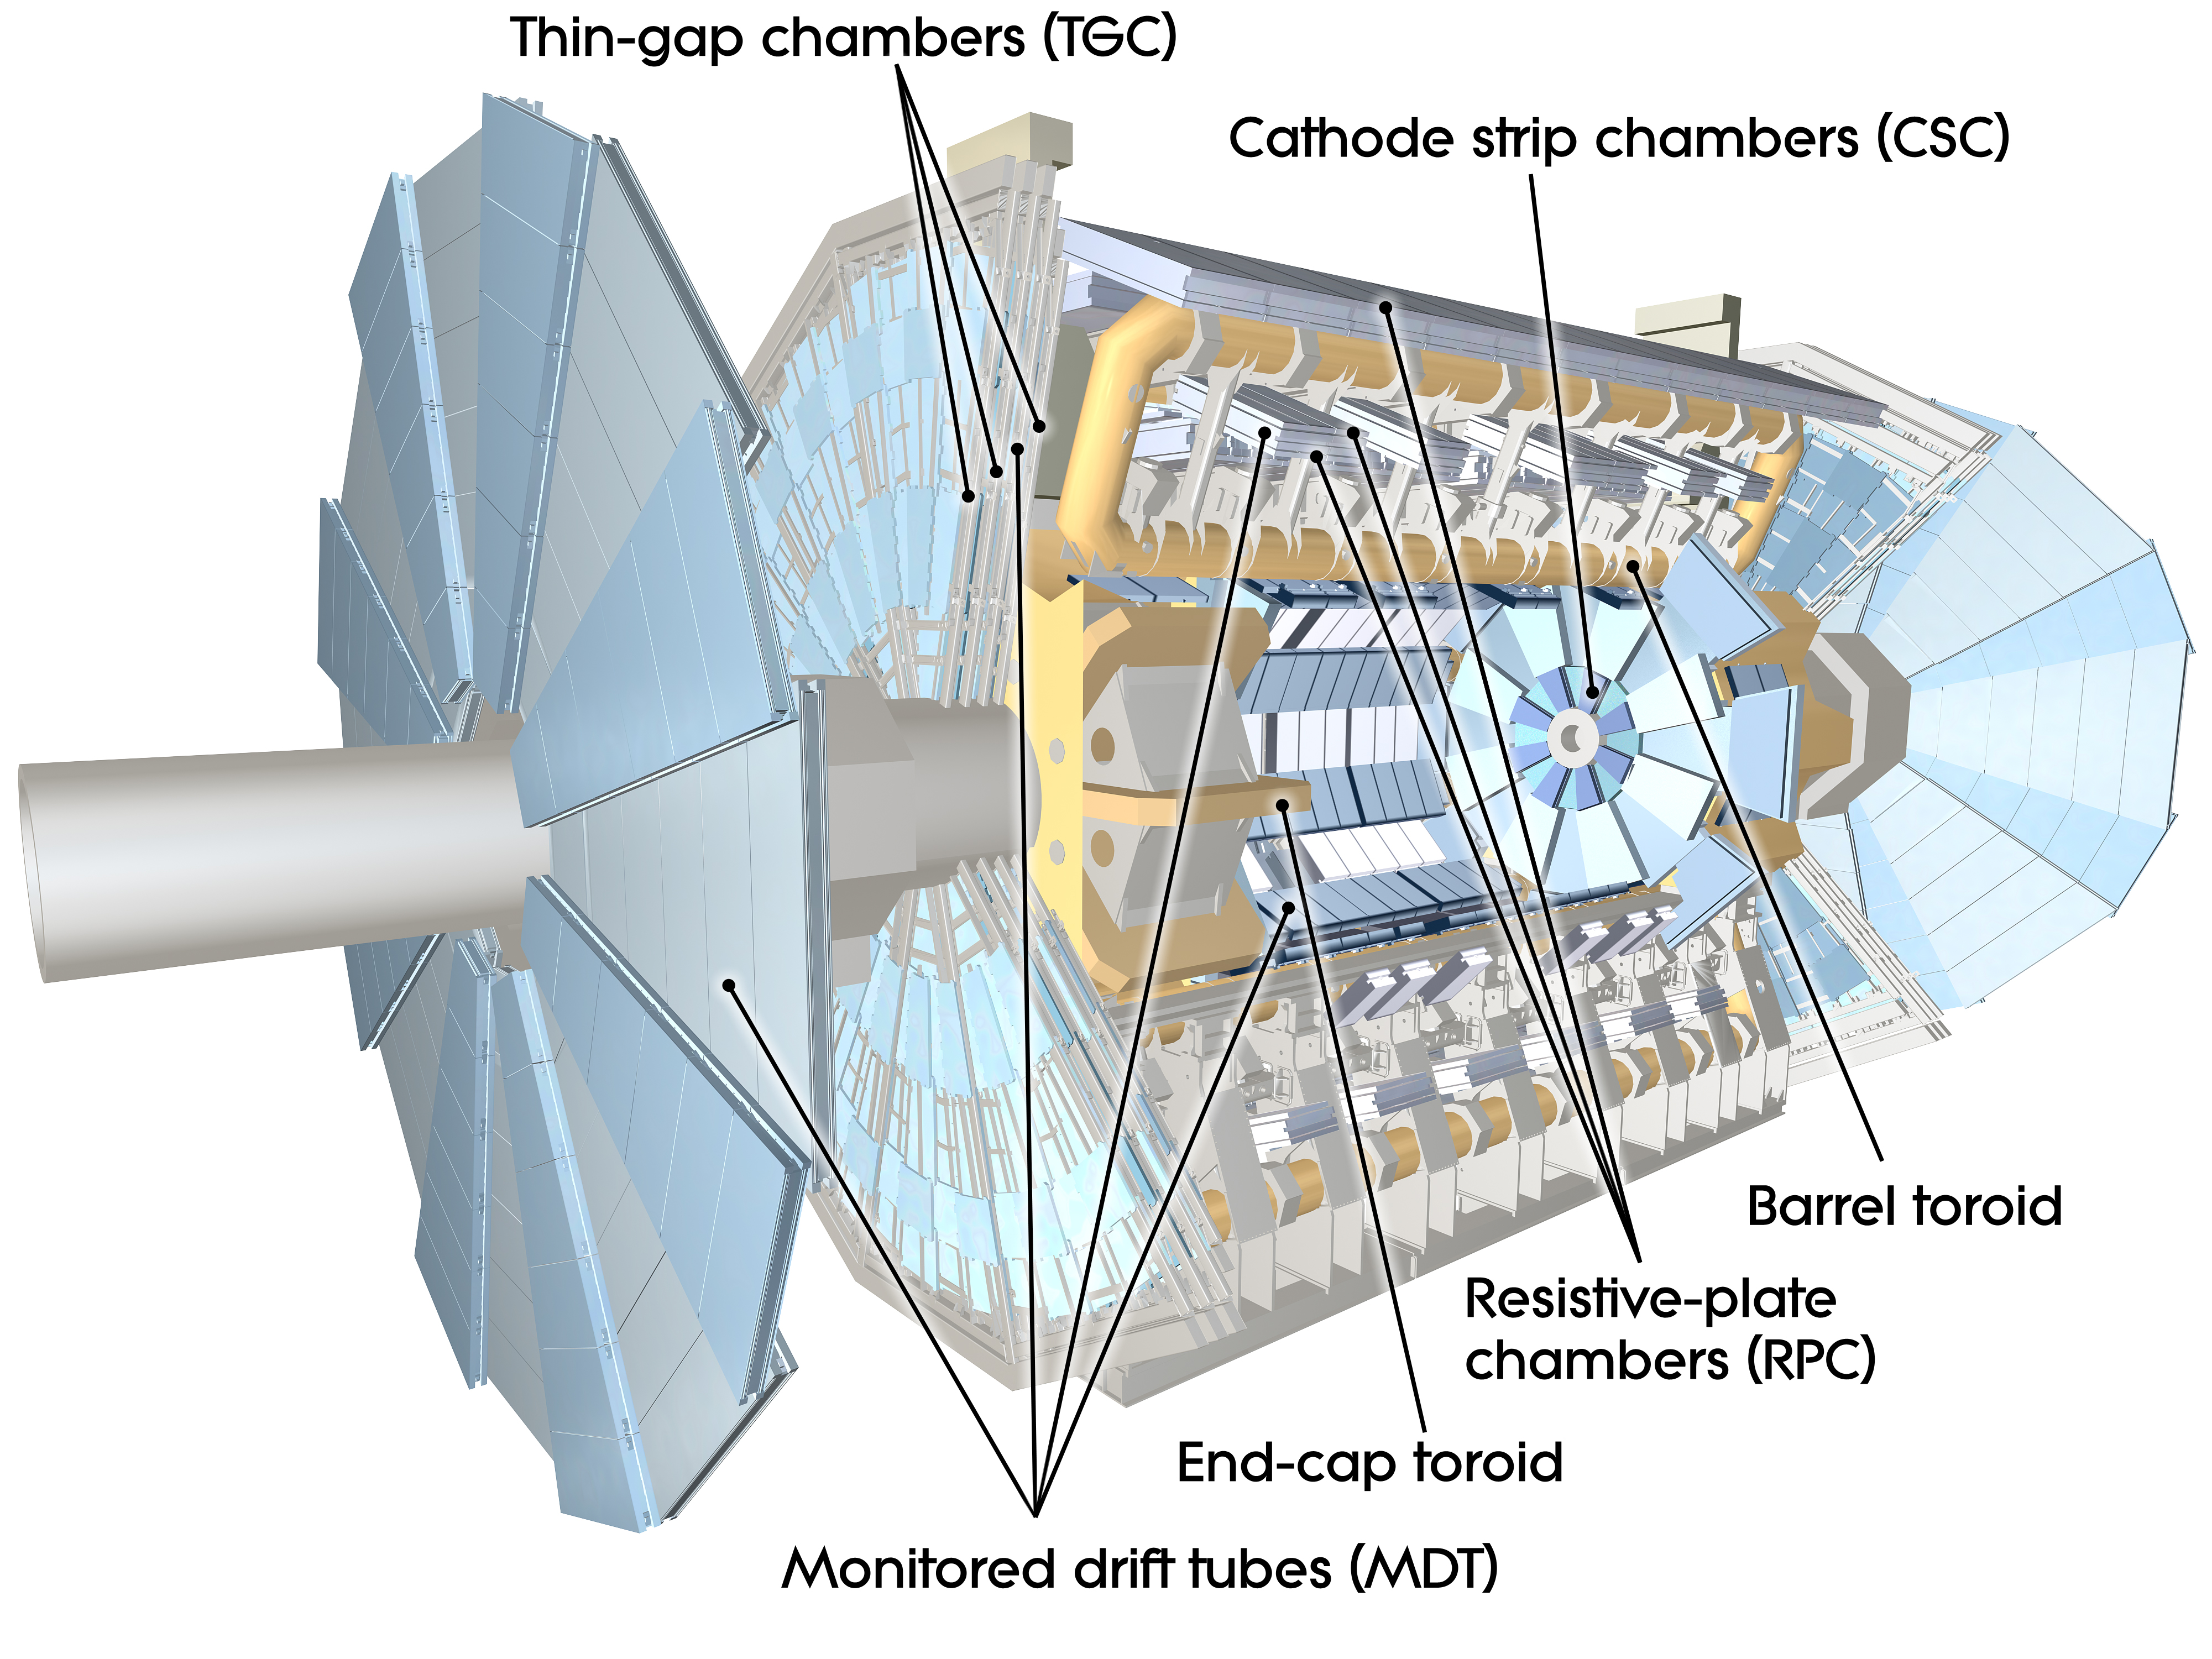
\includegraphics[width=0.9\linewidth]{ms_atlas.png}
    \caption{Cutaway representation of the ATLAS Muon Spectrometer~\cite{ATLAS_run3}.}
    \label{fig:ms_atlas}
\end{figure}

%xxxxxxxxxxxxxxxxxxxxxxxxxxxxxxxxxxxxxxxxxxxxxxxxxxxxxx
\subsection{Forward detectors}
\label{sec:fwd}
%xxxxxxxxxxxxxxxxxxxxxxxxxxxxxxxxxxxxxxxxxxxxxxxxxxxxxx

Beyond the main subsystems listed above, ATLAS employs four compact forward subsystems covering the remaining region of the detector $(|\eta| > 5)$.
LUCID~\cite{Jenni:721908} (LUminosity Cherenkov Integrating Detector), situated $\pm17$~m away from the interaction point, samples inelastic proton-proton interactions at very small angles and provides the experiment’s primary online and offline relative-luminosity measurement.  
LUCID is calibrated thanks to ALFA~\cite{Khalek_2016} (Absolute Luminosity For ATLAS), positioned inside Roman-pot stations $\pm240$ m from the IP, consists of scintillating-fibre tracking modules that can approach the beam to within $\sim\!1$ mm, enabling precise absolute-luminosity determinations and studies of elastic scattering.  
The AFP~\cite{Adamczyk:2015cjy} (ATLAS Forward Proton detector) was the last addition, located at 204 and 217 meters from the interaction point of both sides of the detector and aiming to extend the ATLAS physics reach by trying to tag very forward protons and enabling the observation of different processes where one of the two protons remains untouched.
Finally, the Zero Degree Calorimeter (ZDC)~\cite{Jenni:1009649}, installed $\pm140$ m from the IP, is built from alternating tungsten plates and quartz rods.  Covering $|\eta| > 8.3$, it detects neutral particles at zero degrees and is crucial for centrality measurements in heavy-ion collisions.

%xxxxxxxxxxxxxxxxxxxxxxxxxxxxxxxxxxxxxxxxxxxxxxxxxxxxxx
\subsection{Trigger and Data Acquisition}
\label{sec:trigger}
%xxxxxxxxxxxxxxxxxxxxxxxxxxxxxxxxxxxxxxxxxxxxxxxxxxxxxx
One of the most demanding challenges for an experiment such as ATLAS at the LHC is to devise an efficient strategy for handling the enormous volume of data recorded in the tiny interval that follows each proton-proton collision. During routine LHC operation, proton bunches cross every 25 ns, yielding a raw collision rate of 40 MHz. Since each interaction produces thousands of particles, together with their consequent showers, a single fully digitised ATLAS event occupies roughly 1.5 MB, which would translate into a data stream of about 60 TB s$^{-1}$. Practical bandwidth and storage constraints therefore make it impossible to archive every event, and, in any case, the majority are not relevant to the core physics goals of the experiment. To manage this data stream while retaining the maximum amount of useful information, ATLAS employs a dedicated trigger system~\cite{trigger_run2}. During Run-2 the trigger chain comprised two levels: a hardware-based Level-1 (L1) trigger, followed by a software-based High-Level Trigger (HLT). A schematic overview of the ATLAS Trigger and Data-Acquisition (TDAQ) system for Run-2 is shown in Figure~\ref{fig:trigger_system}.
\begin{figure}[htbp]
    \centering
        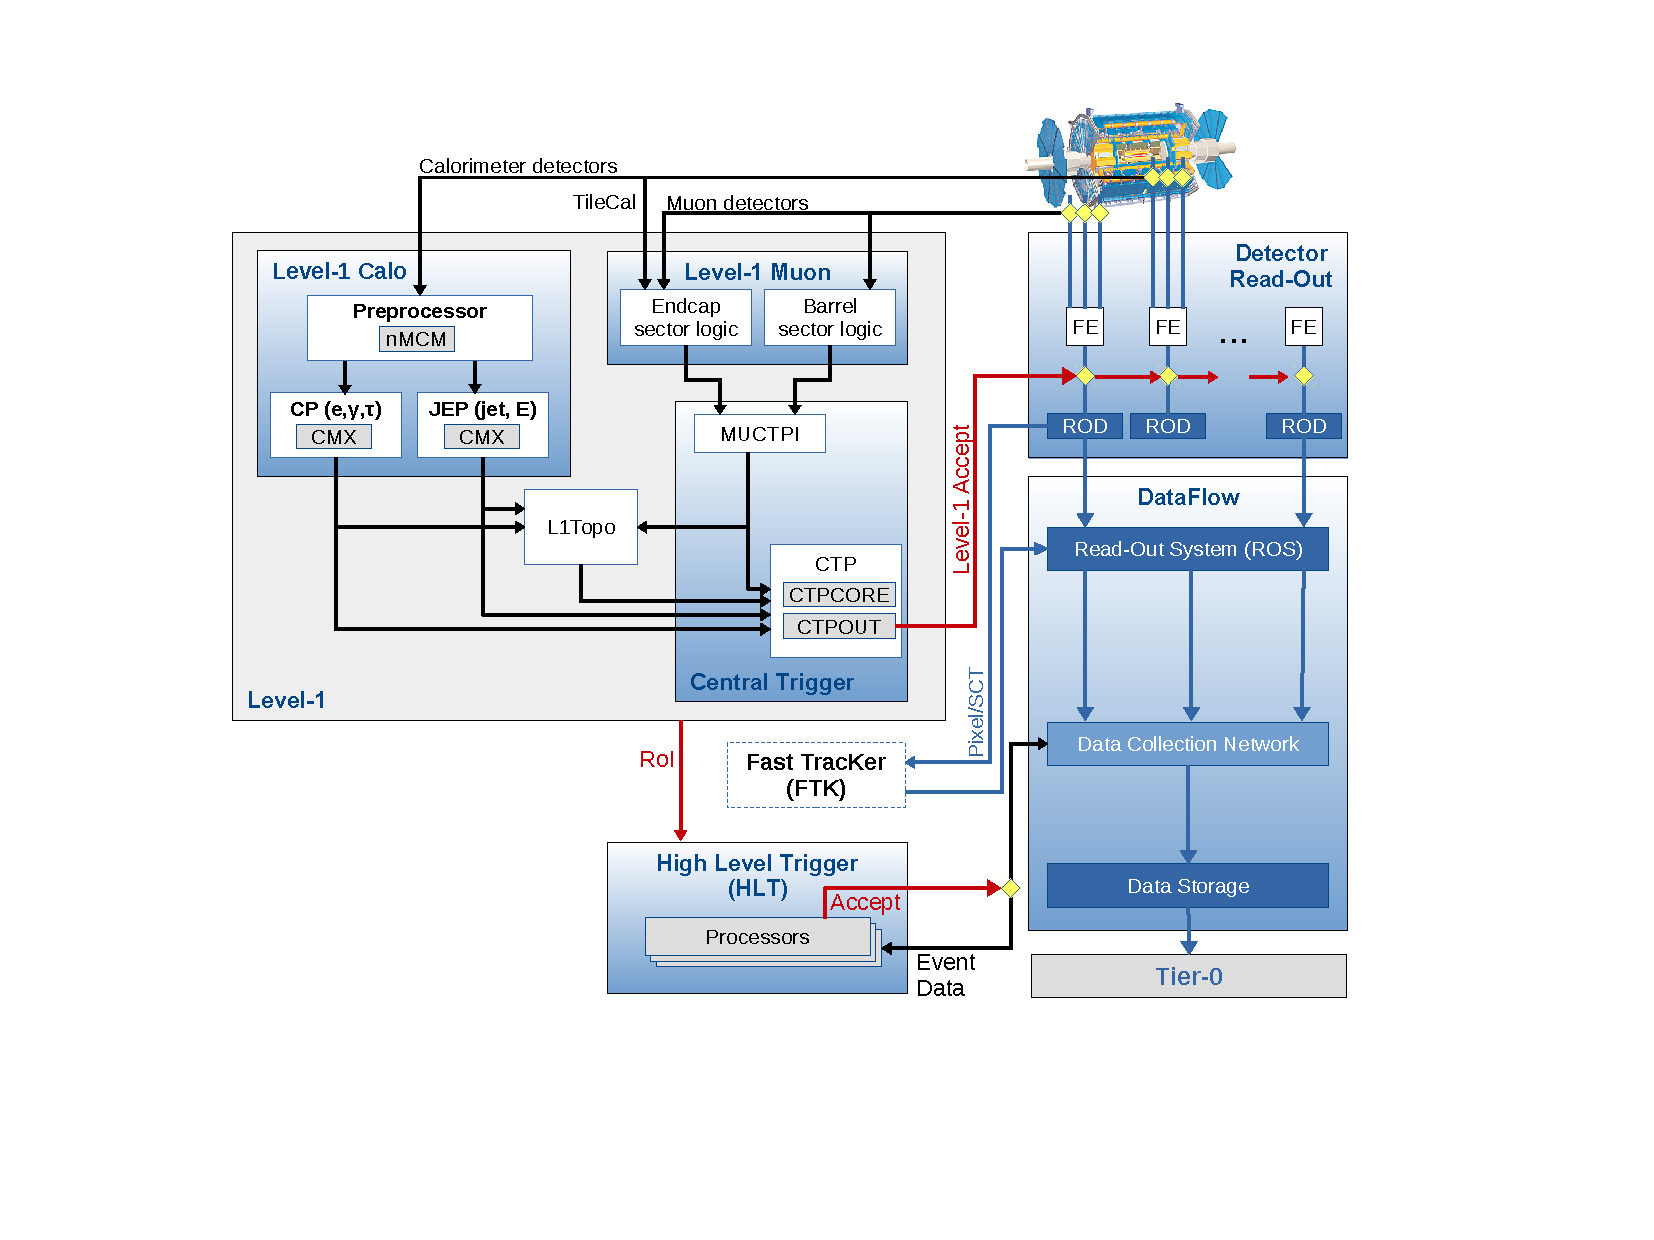
\includegraphics[width=0.75\linewidth]{tdaq-run2.pdf}
    \caption{Schematic of the ATLAS Trigger and Data Acquisition system in Run-2 with specific focus given to the components of the L1 Trigger system~\cite{atlas_daq_run2}.}
    \label{fig:trigger_system}
\end{figure}

The Level-1 trigger is a hardware-based system that reduces the raw 40 MHz collision rate down to about 100 kHz, operating with an exceptionally short latency of roughly 2.5 µs thanks to purpose-built custom and commercial electronics. The front-end electronics of every sub-detector store data in on-chip pipeline memories at the full 40 MHz bunch-crossing frequency. These buffers keep the digitised samples for ∼25 µs, that is the fixed window within which the L1 decision must be issued. That decision relies exclusively on information from the calorimeters and the muon spectrometer.

The L1 Calorimeter (L1Calo) trigger uses coarsened calorimeter read-outs (trigger towers) to locate regions of high energy deposition, i.e.\ regions of interest (RoIs). The L1 Muon (L1Muon) trigger exploits hits in the RPCs and TGCs to flag muon candidates, estimate their transverse momentum, and assign them to the correct bunch crossing. Outputs from L1Calo and L1Muon are merged in the Central Trigger Processor (CTP), which delivers the final verdict. If an event is accepted (an L1-Accept, or L1A), a signal is sent back to the front-end electronics so that the complete data corresponding to that bunch crossing can be read out from the pipeline memories.

The events accepted at Level-1 are first formatted by the sub-detector Read-Out Drivers (RODs) and then forwarded to the software-based High-Level Trigger (HLT). Running on a large computer farm, the HLT performs a rapid, partial reconstruction-tracking, charged-particle and jet identification (including $b$-jets), and a first estimate of the missing transverse momentum, throttling the event stream from $100$~kHz to roughly $1$~kHz. Events that satisfy these online selections are written to permanent storage and transmitted to CERN’s Tier-0 centre for full offline reconstruction. While awaiting the HLT decision, the corresponding data fragments remain buffered in the Read-Out System (ROS).

During LS2, the Phase-I upgrade preserved the two-level architecture while introducing a suite of crucial improvements. A fully digital L1Calo trigger path now feeds three FPGA-based feature extractors: eFEX for electrons and photons, jFEX for jets and missing transverse energy, and gFEX for global event variables. It uses super-cell granularity as fine as $\Delta\eta\times\Delta\phi = 0.025\times0.025$. In the forward region $(1.3<|\eta|<2.4)$ the newly installed NSW provide high-resolution muon trigger primitives, tightening transverse-momentum thresholds and cutting fake rates. The refurbished Level-1 Topological Processor exploits the finer calorimeter and muon inputs to impose angular, invariant-mass and transverse-mass selections in hardware. At the second stage, the HLT farm now runs on expanded computing resources, maintaining an output of roughly 3 kHz at an average event size of about 2.1 MB.

%The Phase-II TDAQ upgrade, developed for the new conditions that will be delivered by HL-LHC, therefore foresees a two-stage hardware trigger in which an initial Level-0 decision accepts events at roughly \SI{1}{\mega\hertz}, followed by a refined Level-1 selection that throttles the rate to about \SI{400}{\kilo\hertz}. Both stages will exploit full-granularity calorimeter read-outs together with prompt track information from the new ITk. The latency budget will be stretched to $\sim!\SI{10}{\micro\second}$, and a trigger-less streaming DAQ is foreseen, capable of digesting data throughputs in excess of \SI{5}{\tera\byte\per\second}. An enlarged processing farm, augmented with hardware accelerators such as FPGAs and GPUs, will then filter the stream down to a sustainable output of \SIrange{10}{15}{\kilo\hertz} for permanent storage. Collectively, these upgrades will preserve and probably extend the experiment’s physics reach in the demanding high-pile-up environment of the HL-LHC.

%xxxxxxxxxxxxxxxxxxxxxxxxxxxxxxxxxxxxxxxxxxxxxxxxxxxxxx
\subsection{ATLAS software and data-processing framework}
\label{sec:athena}
%xxxxxxxxxxxxxxxxxxxxxxxxxxxxxxxxxxxxxxxxxxxxxxxxxxxxxx

It is worth clarifying at this point, for later reference throughout the thesis, the role of the ATLAS software infrastructure. The ATLAS software is divided into two main branches, built and distributed in several packages or projects available on CERN \textsc{gitlab}. On one hand, \textsc{athena}~\cite{athena} constitutes the offline framework used for simulation, reconstruction and analysis of both real and simulated data. On the other hand, the TDAQ~\cite{tdaq} software is responsible for the online operation of the experiment, managing the trigger system and data flow during collisions. 

Different releases of the \textsc{athena} software are typically made available during the processing of the dataset of each data acquisition run. During Run-2, the principal release in use was release 21 (rel.21), which supported the reconstruction of data collected as well as the associated simulation campaigns MC16a (corresponding to the 2015-2016 data taking years), MC16d (2017) and MC16e (2018). 

Towards the end of Run-2, a new version of \textsc{athena} (release 22, rel.22) was developed in order to reprocess the full Run-2 dataset. The new release introduced significant improvements with respect to R.21, such as more advanced reconstruction algorithms, enhanced Inner Detector tracking, updated MC simulation and improved memory efficiency. This ensured a uniform and higher-quality reconstruction of Run-2 data (campaigns MC20a, MC20d and MC20e), while at the same time establishing the framework to be employed for Run-3.

For Run-3, \textsc{athena} R.22 continues to be the basis for both data-taking and MC simulation. The corresponding campaigns are labelled MC23a (2022), MC23d (2023) and MC23e (2024). This naming convention is used consistently throughout the thesis when referring to Monte Carlo samples corresponding to different data-taking years. A summary of the relevant releases and their associated campaigns is provided in Table~\ref{tab:athena_mc_campaigns}.

\begin{table}[htbp]
    \centering
    \small
    \renewcommand{\arraystretch}{1.3} % aumenta el espacio vertical entre filas
    \setlength{\tabcolsep}{12pt}      % aumenta el espacio horizontal entre columnas
    \caption{Summary of ATHENA releases and the corresponding Monte Carlo campaigns associated with each data-taking year in Run-2 and Run-3.}
    \label{tab:athena_mc_campaigns}
    \begin{tabular}{lcc}
        \hline
        \textbf{Data-taking Year} & \textbf{Release 21} & \textbf{Release 22} \\
        \hline
        2015--2016 & MC16a & MC20a \\
        2017       & MC16d & MC20d \\
        2018       & MC16e & MC20e \\
        \hline
        2022       & --    & MC23a \\
        2023       & --    & MC23d \\
        2024       & --    & MC23e \\
        \hline
    \end{tabular}
\end{table}



%xxxxxxxxxxxxxxxxxxxxxxxxxxxxxxxxxxxxxxxxxxxxxxxxxxxxxx
\subsection{Detector Control Systems}
\label{sec:dcs}
%xxxxxxxxxxxxxxxxxxxxxxxxxxxxxxxxxxxxxxxxxxxxxxxxxxxxxx
A smooth dialogue between all ATLAS subsystems and the technical infrastructure that steers them is essential for reliable detector operation and data flow. This coordination is handled by the Detector Control System (DCS)~\cite{atlas_DCS}, which provides a unified interface for operators and continuously monitors voltages, temperatures, gas flows, and countless other parameters. Whenever an abnormal condition is detected, the DCS automatically issues alarms, attempts corrective actions where possible, and guides shifters through any manual interventions required. In addition, the DCS exchanges status flags with the TDAQ so that data taking proceeds only when all components are in a safe, ready state, and it brokers communication among subsystems that are controlled independently.

%xxxxxxxxxxxxxxxxxxxxxxxxxxxxxxxxxxxxxxxxxxxxxxxxxxxxxx
\subsection{The LHC computer grid}
\label{sec:computer_grid}
%xxxxxxxxxxxxxxxxxxxxxxxxxxxxxxxxxxxxxxxxxxxxxxxxxxxxxx
To explain how the events accepted by the trigger are eventually processed, one must introduce The Worldwide LHC Computing Grid (WLCG)~\cite{Bird:1695401}, which is a global, tiered infrastructure that stores, distributes and processes the multi-petabyte data stream produced by the LHC experiments.  Data first reach Tier-0 at CERN, where the raw 1~kHz detector output is buffered, reconstructed and replicated; CERN then distributes this primary dataset to thirteen Tier-1 centres on three continents for large-scale reprocessing and long-term archival. Roughly 170 Tier-2 sites (university and regional clusters) supply the bulk of CPU for user analyses and Monte-Carlo production, while a large number local Tier-3 farms serve individual groups.  
Today the WLCG federates $\sim$1.4 million CPU cores and $\sim$1.5 EB of disk and tape across 42 countries, sustaining average data‐transfer rates above 260 GB s$^{-1}$ and executing in excess of two million grid jobs daily.  This distributed model enables more than 1200 physicists to access ATLAS data quasi-real-time, making large-scale analysis feasible without centralised super-computing resources.
